\documentclass[12pt]{article}

\usepackage{sbc-template}

\usepackage{graphicx,url}

\usepackage[utf8]{inputenc}  
\usepackage[brazil]{babel}   

\graphicspath{ {./img/} }
     
\sloppy

\title{Estudo Comparativo de Mecanismos de Segurança Aplicados à Autenticação e Autorização em Sistemas Web}

\author{Rafael Strack\inst{1}, Adriano Ferrasa\inst{1}}


\address{Departamento de Informática -- Universidade Estadual de Ponta Grossa
  (UEPG)\\
  84.030-900 -- Ponta Grossa -- PR -- Brasil
\email{rafa\_strack@hotmail.com, ferrasa@uepg.br}
}
\begin{document}

\maketitle

\begin{abstract}
This article presents a comparative study of authentication and authorization 
mechanisms in web systems, aiming to provide an in-depth analysis of the 
available options and their characteristics. The study describes the most 
commonly used methods such as passwords, tokens, multifactor authentication, 
and OAuth, analyzing their advantages and disadvantages. Additionally, 
sequence diagrams are provided to illustrate the usage flow of each method. 
Finally, a comparison of the studied methods is conducted, evaluating their 
effectiveness in terms of security. Proper understanding of these mechanisms 
is crucial to ensure the security of web systems and guide the correct 
choice in future projects.
\end{abstract}
     
\begin{resumo}
Este artigo apresenta um estudo comparativo dos mecanismos de autenticação 
e autorização em sistemas web, visando fornecer uma análise aprofundada das 
opções disponíveis e suas características. O estudo descreve os métodos mais 
utilizados, como senhas, tokens, autenticação multifator e OAuth, analisando 
suas vantagens e desvantagens. Além disso, são apresentados diagramas de 
sequência para ilustrar o fluxo de utilização de cada método. Ao final, é 
realizada uma comparação dos métodos estudados, avaliando sua eficácia em 
termos de segurança. A compreensão adequada desses mecanismos é fundamental 
para garantir a segurança dos sistemas web e orientar a escolha correta em 
projetos futuros.
\end{resumo}


\section{Introdução}

Com a expansão da internet, os sistemas web assumiram um papel crucial no
cotidiano de bilhões de pessoas em todo o mundo. Desde o uso de redes sociais até
o gerenciamento de negócios online, essas ferramentas se tornaram indispensáveis
para diversas atividades. Tanto pessoas físicas quanto empresas dependem desses
sistemas para garantir a eficiência e produtividade de suas operações. No entanto, a
segurança desses sistemas é uma preocupação constante para desenvolvedores e
usuários, pois há uma série de ameaças e vulnerabilidades que podem comprometer
sua integridade.

A fundação OWASP (\emph{Open Worldwide Application Security Project}) atualiza
regularmente um relatório chamado OWASP Top 10, onde são descritos os 10 riscos
de segurança mais críticos em sistemas web. Na última edição, realizada em 2021, a
categoria que ficou em primeira colocação foi a quebra de controle de acesso. Em
sétima colocação, ficou a categoria de falhas de identificação e autenticação 
\cite{OWASP2021}. Esses problemas são diretamente relacionados aos processos de 
autenticação e autorização de usuários, os quais são essenciais para garantir a 
proteção adequada dos sistemas.

De modo geral, a autenticação é o processo de validação de usuários, enquanto a 
autorização é o método que fornece as permissões de acesso corretas aos recursos 
para usuários previamente autenticados \cite{TUMIN2012}. Atualmente, existem diversos 
mecanismos de autenticação e autorização de usuários disponíveis, como senhas, \emph{tokens}, 
autenticação multifator, OAuth, OpenID, entre outros. Cada um desses mecanismos 
apresenta características distintas, pontos positivos e negativos, sendo fundamental 
garantir a correta implementação dos mecanismos escolhidos, de forma a assegurar a 
efetividade da segurança dos sistemas web. 

Diante desse contexto, o presente trabalho tem como objetivo realizar um estudo 
comparativo dos diferentes mecanismos de autenticação e autorização, com o propósito 
de fornecer uma análise aprofundada que auxilie na escolha adequada desses mecanismos 
em projetos de sistemas web. O estudo visa oferecer uma compreensão ampla das 
características, pontos fortes e limitações de cada mecanismo, permitindo a seleção 
correta e a implementação eficiente das medidas de segurança necessárias.

\section{Autenticação e Autorização}

Na maioria dos sistemas web, é necessário realizar um controle de acesso, para que somente
certos usuários possam acessar recursos protegidos. Para isso, o mecanismo  de controle de 
acesso depende de dois processos relacionados: a autenticação e a autorização 
\cite{SULLIVAN2011}.

A autenticação pode ser definida como o processo de confirmação de identidade. Em sistemas web,
devido a falta de conhecimento do mundo real, este processo pode não ser simples 
\cite{CHAPMAN2012}. Existem três grupos de fatores amplamente utilizados para confirmar a 
identidade de um usuário: algo que o usuário sabe, algo que o usuário é e algo que o usuário 
possui. No primeiro grupo, inclui-se as senhas, PINs (\emph{Personal Identification Number}) e 
frases secretas. No segundo grupo, inclui-se certificados digitais, \emph{smart cards} e 
\emph{tokens} de segurança. O terceiro grupo inclui técnicas biométricas, como como impressões 
digitais, reconhecimento facial ou de voz, entre outras \cite{SULLIVAN2011}.

A autorização é o processo pelo qual o sistema decide se um usuário previamente autenticado 
possui permissão para acessar um recurso ou executar uma determinada ação \cite{SPILCA2020}.

\noindent [...]

% arrumar, complementar, procurar mais referencias sobre a definição de autorização e seus tipos

% Esta autorização pode ser feita baseada em usuários, garantindo acesso aos recursos do sistema 
% web para cada usuário de forma distinta, ou baseada em perfis (\emph{roles}), em que cada usuário
% possui um perfil, e cada perfil tem diferentes níveis de acesso aos recursos do sistema.


\subsection{HTTP Basic Authentication}

A HTTP (\emph{Hypertext Transfer Protocol}) Basic Authentication foi definida na especificação 
RFC 2617 \cite{RFC2617} e atualizada na RFC 7617 \cite{RFC7617}. Neste tipo de autenticação, o servidor
web recusa uma transação caso o cliente não esteja autenticado, desafiando-o para obter um nome de usuário
e senha válidos. Este desafio de autenticação é iniciado retornando o status HTTP 401 (não autorizado) e
especificando o domínio de segurança (\emph{security realm}) a ser acessado, com o cabeçalho WWW-Authenticate.
Ao receber o desafio, o navegador abre uma caixa de diálogo para que o usuário insira as credenciais para 
acesso ao domínio. O navegador então junta as informações de usuário e senha, colocando dois pontos entre eles,
e os codifica usando o método de codificação base-64. Estas credenciais codificadas são colocadas no cabeçalho
Authorization, e então a requisição é enviada para o servidor, que fará a validação das credenciais e, caso
validadas, retorna-se o status HTTP 200 (OK), e as informações da página web requisitada \cite{GOURLEY2002}.
Um exemplo do funcionamento deste método de autenticação é mostrado na Figura \ref{fig:basicAuth}.

% Os domínios de segurança utilizados por essa autenticação são identificadores de coleções de recursos, geralmente
% que possuem alguma relação ou mesmo nível de proteção. Estes domínios, incorporados ao cabeçalho HTTP, definem
% quais recursos o usuário, ao ser autenticado, terá acesso. 

\begin{figure}[ht]
  \centering
  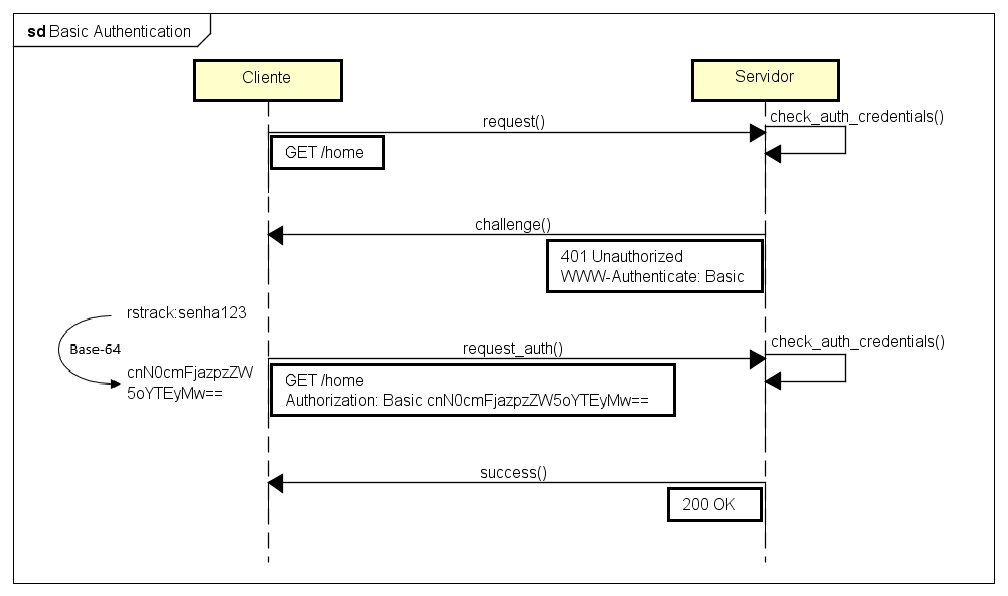
\includegraphics[width=1\textwidth]{Basic Authentication.png}
  \caption{Exemplo de HTTP Basic Authentication}
  \label{fig:basicAuth}
\end{figure}

A diretiva de domínio (\emph{realm}) utilizada na Basic Authentication define os espaços de proteção do sistema 
web. Esses domínios permitem que os recursos protegidos sejam particionados, cada um com seu próprio esquema de 
autenticação e/ou autorização \cite{RFC2617}.

A HTTP Basic Authentication é simples e de fácil implementação, porém não possui segurança. As credenciais do
usuário podem ser facilmente decodificadas, visto que a codificação base64 é facilmente reversível, podendo ser
realizada em poucos segundos. Também é possível realizar ataques de reprodução, visto que terceiros podem capturar
pacotes e replicá-los, mesmo que codificados, podendo obter acesso ao sistema. Este tipo de autenticação não possui
proteção contra \emph{proxies} ou \emph{middlewares}, que podem facilmente modificar o corpo da mensagem, e também
são vulneráveis a servidores falsificados, que se passam por outros para realizar o roubo de credenciais. Além Estes
pontos negativos a autenticação básica não possui encerramento de sessão, fazendo com que o usuário permaneça conectado
até o fechamento do navegador.

\subsection{HTTP Digest Authentication}
\
\subsection{Session-Based Authentication}
\
\subsection{Token-Based Authentication}
\
\subsection{OAuth e OAuth2}
\
\subsection{OpenID}
\
\section{Materiais e Métodos}
\
\section{Resultados e Discussão}
\
\section{Conclusão}
\
% \section{First Page} \label{sec:firstpage}

% The first page must display the paper title, the name and address of the
% authors, the abstract in English and ``resumo'' in Portuguese (``resumos'' are
% required only for papers written in Portuguese). The title must be centered
% over the whole page, in 16 point boldface font and with 12 points of space
% before itself. Author names must be centered in 12 point font, bold, all of
% them disposed in the same line, separated by commas and with 12 points of
% space after the title. Addresses must be centered in 12 point font, also with
% 12 points of space after the authors' names. E-mail addresses should be
% written using font Courier New, 10 point nominal size, with 6 points of space
% before and 6 points of space after.

% The abstract and ``resumo'' (if is the case) must be in 12 point Times font,
% indented 0.8cm on both sides. The word \textbf{Abstract} and \textbf{Resumo},
% should be written in boldface and must precede the text.

% \section{CD-ROMs and Printed Proceedings}

% In some conferences, the papers are published on CD-ROM while only the
% abstract is published in the printed Proceedings. In this case, authors are
% invited to prepare two final versions of the paper. One, complete, to be
% published on the CD and the other, containing only the first page, with
% abstract and ``resumo'' (for papers in Portuguese).

% \section{Sections and Paragraphs}

% Section titles must be in boldface, 13pt, flush left. There should be an extra
% 12 pt of space before each title. Section numbering is optional. The first
% paragraph of each section should not be indented, while the first lines of
% subsequent paragraphs should be indented by 1.27 cm.

% \subsection{Subsections}

% The subsection titles must be in boldface, 12pt, flush left.

% \section{Figures and Captions}\label{sec:figs}


% Figure and table captions should be centered if less than one line, otherwise justified and indented by 0.8cm on
% both margins, as shown in Figure. The caption font must
% be Helvetica, 10 point, boldface, with 6 points of space before and after each
% caption.


% In tables, try to avoid the use of colored or shaded backgrounds, and avoid
% thick, doubled, or unnecessary framing lines. When reporting empirical data,
% do not use more decimal digits than warranted by their precision and
% reproducibility. Table caption must be placed before the table (see Table 1)
% and the font used must also be Helvetica, 10 point, boldface, with 6 points of
% space before and after each caption.

% \section{Images}

% All images and illustrations should be in black-and-white, or gray tones,
% excepting for the papers that will be electronically available (on CD-ROMs,
% internet, etc.). The image resolution on paper should be about 600 dpi for
% black-and-white images, and 150-300 dpi for grayscale images.  Do not include
% images with excessive resolution, as they may take hours to print, without any
% visible difference in the result. 

% \section{References}


% The references must be listed using 12 point font size, with 6 points of space
% before each reference. The first line of each reference should not be
% indented, while the subsequent should be indented by 0.5 cm.

\bibliographystyle{sbc}
\bibliography{references}

\end{document}
